\documentclass[11pt,a4paper]{article}

\usepackage[T1]{fontenc}
\usepackage[utf8]{inputenc}
\usepackage{lmodern}
\usepackage[margin=1in]{geometry}
\usepackage{booktabs}
\usepackage{tabularx}
\usepackage{longtable}
\usepackage{xcolor}
\usepackage{fancyhdr}
\usepackage{titlesec}
\usepackage{enumitem}
\usepackage{listings}
\usepackage{tikz}
\usepackage{microtype}
\usepackage{caption}
\usepackage{float}
\usepackage{url}
\usepackage{hyperref}
\usepackage[skip=0.9\baselineskip,indent=0pt]{parskip}
\setlength{\emergencystretch}{3em}

\usetikzlibrary{arrows.meta,positioning,shapes.geometric,calc,fit,backgrounds,decorations.pathreplacing}

% ---------------------------------------------------------------- palette
\definecolor{accent}{HTML}{000000}
\definecolor{accentlight}{HTML}{F0F0F0}
\definecolor{rule}{HTML}{888888}
\definecolor{codebg}{HTML}{F5F6F8}
\definecolor{codekw}{HTML}{000000}
\definecolor{codecm}{HTML}{444444}
\definecolor{warnbg}{HTML}{F0F0F0}
\definecolor{warnrule}{HTML}{000000}

\hypersetup{
  colorlinks=true,
  linkcolor=black,
  urlcolor=black,
  citecolor=black,
  pdftitle={Marconi Research and Innovations Lab: Infrastructure Operations Agent},
  pdfsubject={Design and Implementation},
  bookmarksnumbered=true
}

% ---------------------------------------------------------------- headers
\pagestyle{fancy}
\fancyhf{}
\renewcommand{\headrulewidth}{0pt}
\renewcommand{\footrulewidth}{0pt}
\fancyfoot[C]{\small\thepage}

% ---------------------------------------------------------------- headings
\titleformat{\section}{\Large\bfseries\color{accent}}{\thesection}{0.7em}{}
\titleformat{\subsection}{\large\bfseries\color{accent!85!black}}{\thesubsection}{0.6em}{}
\titleformat{\subsubsection}{\normalsize\bfseries}{\thesubsubsection}{0.6em}{}
\titlespacing*{\section}{0pt}{0pt}{0.9em}

% Every section starts on a fresh page.
\let\stdsection\section
\renewcommand{\section}{\clearpage\stdsection}

\captionsetup{font=small,labelfont={bf,color=accent}}
\setlist[itemize]{itemsep=4pt,topsep=2pt,parsep=0pt,leftmargin=*,align=left}
\setlist[enumerate]{itemsep=4pt,topsep=2pt,parsep=0pt,leftmargin=*,align=left}
\setlist[description]{itemsep=4pt,topsep=2pt,parsep=0pt,leftmargin=0pt,style=unboxed}

% ---------------------------------------------------------------- listings
\lstdefinestyle{plain}{
  basicstyle=\ttfamily\footnotesize,
  backgroundcolor=\color{codebg},
  keywordstyle=\color{codekw}\bfseries,
  commentstyle=\color{codecm}\itshape,
  stringstyle=\color{accent},
  frame=single,
  rulecolor=\color{rule},
  framesep=6pt,
  breaklines=true,
  showstringspaces=false,
  columns=fullflexible,
  xleftmargin=4pt,
  xrightmargin=4pt,
  aboveskip=10pt,
  belowskip=10pt
}
\lstset{style=plain}

% ---------------------------------------------------------------- tikz styles
\tikzset{
  layer/.style={draw=accent, fill=accentlight, rounded corners=2pt,
                minimum height=8mm, text width=0.70\textwidth, align=center,
                font=\small},
  boxn/.style={draw=accent, fill=white, rounded corners=2pt,
               minimum height=8mm, minimum width=22mm, align=center, font=\small},
  statn/.style={draw=accent, fill=accentlight, circle, minimum size=13mm,
                align=center, font=\small},
  term/.style={draw=accent!60, fill=white, rounded corners=6pt,
               minimum size=8mm, align=center, font=\footnotesize},
  fl/.style={-{Stealth[length=2mm]}, draw=accent!80, thick},
  fldash/.style={-{Stealth[length=2mm]}, draw=accent!60, thick, dashed},
  lbl/.style={font=\scriptsize, inner sep=1.5pt, fill=white}
}

\begin{document}

% ================================================================ TITLE + ABSTRACT
\pagenumbering{roman}
\begin{center}
{\Huge\bfseries\color{accent} Marconi Research and Innovations Lab\par}
\vspace{0.5em}
{\LARGE\bfseries Infrastructure Operations Agent\par}
\vspace{0.3em}
{\Large\itshape Design and Implementation\par}
\end{center}
\vspace{1.5em}

\section*{Abstract}
\addcontentsline{toc}{section}{Abstract}
\markboth{Abstract}{}

Diagnosing a fault in a small self-hosted environment usually means opening three
separate interfaces and correlating them by hand: the container runtime for process
state, a metrics server for resource behaviour, and a log store for what the service
itself reported. The work is mechanical, repeats every incident, and takes longest
exactly when an operator can least afford the delay.

This report describes a system that performs that correlation on request. An operator
asks a question in ordinary language from a chat client; a language model, given a
fixed set of read-only query tools, decides which backends to consult, issues the
queries, and returns an answer with the evidence it rests on, a likely cause, and
recommended next steps. The design has one governing constraint: the agent can
observe but cannot act. No tool in the system issues a mutating call to any backend,
so the worst outcome of a mistaken model turn is an incorrect answer rather than a
stopped service --- a guarantee enforced by the set of operations exposed to the model,
not by instructions given to it.

Beyond the conversational path, the system polls container and endpoint health on a
fixed cycle, alerts on transitions, records them durably, and publishes daily and
weekly reports that keep measured data separate from the generated prose summarising
it. The report describes how the system is built and why, and closes with the design
decisions behind it, what each one costs, and the limitations that remain.

\clearpage
\setcounter{tocdepth}{1}
\tableofcontents

\clearpage
\pagenumbering{arabic}

% ================================================================ 1
\section{Introduction}

\subsection{The operational problem}

A small self-hosted environment has three separate sources of truth about its
health: the container runtime (process state), a metrics server (time series), and
a log store (what each service reported). None answers a non-trivial question
alone. Diagnosing a restart needs runtime state, the logs immediately before it,
and the resource curve over the preceding interval, and an experienced operator
runs roughly that sequence for every incident, which branches on what each step
returns and so resists a fixed script.

\subsection{Approach}

The model discovers the environment rather than being told about it: enumeration
operations (services, metric names, label values) exist alongside query operations,
and the model is instructed to enumerate before it queries, since a guessed name
returns nothing.

Access runs through the existing chat workspace rather than a purpose-built
interface, so a question, an alert, and a scheduled report all land in the place an
operator already watches.

\subsection{Scope}

\begin{enumerate}
  \item \textbf{Conversational investigation.} Free-form questions, answered with
        every read-only operation available, context retained per conversation.
  \item \textbf{Structured incident reporting.} The same loop on a fixed template:
        summary, observed behaviour, evidence, likely cause, next steps.
  \item \textbf{Continuous monitoring.} Container and endpoint state polled on a
        fixed cycle; transitions produce alerts and durable records.
  \item \textbf{Scheduled reporting.} Daily and weekly digests of current state and
        the transitions recorded over the window.
\end{enumerate}

\subsection{Out of scope}

\begin{enumerate}
  \item \textbf{No write operations.} Nothing restarts, scales, reconfigures, or
        deletes; the design constraint Section~\ref{sec:readonly} enforces.
  \item \textbf{Single tenant.} One environment, one chat workspace, no per-user
        authorisation beyond what the workspace provides.
  \item \textbf{No alerting rule engine.} Alerts fire on state transitions, not
        threshold expressions; metrics feed diagnosis only (Section~\ref{sec:socket-vs-query}).
  \item \textbf{No model training.} The model is an external service reached over
        a network API.
\end{enumerate}

% ================================================================ 2
\subsection{System overview}

The system runs as a single long-lived process: a chat connection, a reasoning loop
that answers questions, a polling loop that watches health, and a scheduled report
task. Figure~\ref{fig:overview} shows the arrangement.

\begin{figure}[H]
\centering
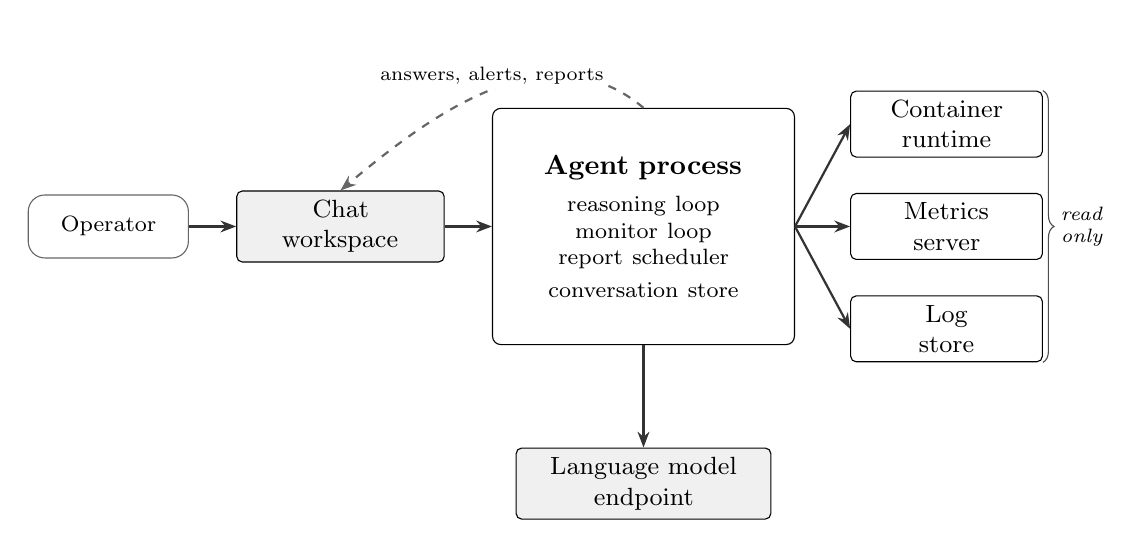
\begin{tikzpicture}[node distance=5mm]

\node[term, text width=18mm] (op) {Operator};
\node[boxn, right=6mm of op, text width=24mm, fill=accentlight] (chat) {Chat\\workspace};

\node[draw=accent, fill=white, rounded corners=3pt, right=6mm of chat,
      text width=36mm, minimum height=30mm, align=center] (proc)
      {\textbf{Agent process}\\[4pt]
       \footnotesize reasoning loop\\
       \footnotesize monitor loop\\
       \footnotesize report scheduler\\
       \footnotesize conversation store};

\node[boxn, right=7mm of proc, yshift=13mm, text width=22mm] (dock) {Container\\runtime};
\node[boxn, right=7mm of proc, text width=22mm] (prom) {Metrics\\server};
\node[boxn, right=7mm of proc, yshift=-13mm, text width=22mm] (loki) {Log\\store};

\node[boxn, below=13mm of proc, text width=30mm, fill=accentlight] (llm) {Language model\\endpoint};

\draw[fl] (op) -- (chat);
\draw[fl] (chat) -- (proc);
\draw[fl] (proc.east) -- (dock.west);
\draw[fl] (proc.east) -- (prom.west);
\draw[fl] (proc.east) -- (loki.west);
\draw[fl] (proc) -- (llm);

\draw[decorate, decoration={brace, amplitude=4pt}, draw=accent!70]
      (dock.north east) -- (loki.south east)
      node[midway, right=3pt, font=\scriptsize\itshape, align=left] {read\\only};

\draw[fldash] (proc.north) to[out=140,in=40] node[lbl,above]{answers, alerts, reports} (chat.north);


\end{tikzpicture}
\caption{Top level arrangement. The agent process is the only component that talks to
both the chat workspace and the observability backends. All backend access is read
only.}
\label{fig:overview}
\end{figure}

\subsubsection{The conversational path}

A slash command, direct message, or mention all reach the same reasoning loop:
consult the model, execute the requested operations, feed back the results, repeat
until it answers without requesting more. The answer is reformatted for the
platform and split across messages past the length limit.

\subsubsection{The monitoring path}

A polling task on a fixed interval reads container state and probes each
configured endpoint, comparing against the last cycle. A change (running/not,
reachable/not) is a transition: logged durably and posted as an alert, with
recoveries on a separate channel.

\subsubsection{The reporting path}

A scheduled task fires daily, rendering current state and the day's transitions,
plus a weekly roll-up of per-service outage counts and downtime on one configured
weekday. Where the publish channel is a forum, each digest opens its own thread.

% ================================================================ 3
\section{Architecture}

\subsection{Layering}

The system is arranged in layers with imports running strictly downward
(Figure~\ref{fig:layers}); each is defined as much by what it refuses to know as
by what it does.

\begin{figure}[H]
\centering
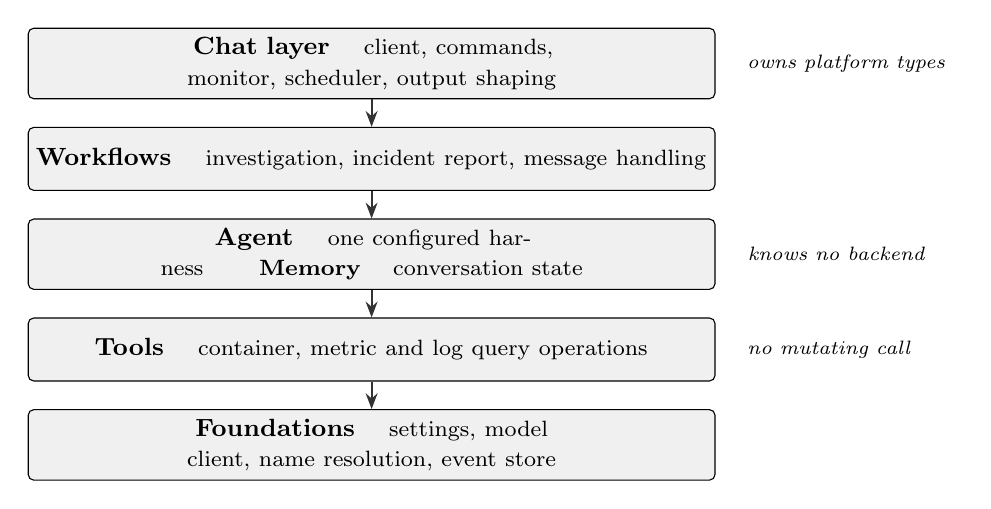
\begin{tikzpicture}[node distance=3.5mm]

\node[layer] (l1) {\textbf{Chat layer} \quad\footnotesize client, commands, monitor, scheduler, output shaping};
\node[layer, below=of l1] (l2) {\textbf{Workflows} \quad\footnotesize investigation, incident report, message handling};
\node[layer, below=of l2] (l3) {\textbf{Agent} \quad\footnotesize one configured harness \qquad \textbf{Memory} \quad\footnotesize conversation state};
\node[layer, below=of l3] (l4) {\textbf{Tools} \quad\footnotesize container, metric and log query operations};
\node[layer, below=of l4] (l5) {\textbf{Foundations} \quad\footnotesize settings, model client, name resolution, event store};

\draw[fl] (l1) -- (l2);
\draw[fl] (l2) -- (l3);
\draw[fl] (l3) -- (l4);
\draw[fl] (l4) -- (l5);

\node[right=3mm of l1, font=\scriptsize\itshape, text width=26mm, align=left] {owns platform types};
\node[right=3mm of l3, font=\scriptsize\itshape, text width=26mm, align=left] {knows no backend};
\node[right=3mm of l4, font=\scriptsize\itshape, text width=26mm, align=left] {no mutating call};

\end{tikzpicture}
\caption{Layering. Imports run downward only. The agent sits below the workflows that
call it and above the tools it is constructed with.}
\label{fig:layers}
\end{figure}

\subsubsection{Foundations}

Settings read configuration from the environment once at import into a validated,
typed object, resolving both storage paths so every component agrees which file is
which. It also derives the model identifier (a \texttt{provider:model} string) and
publishes the credential and endpoint to the process environment, so any server
speaking the OpenAI-compatible protocol~\cite{openai} is usable, including a
self-hosted model. Name resolution provides the one matching rule used for every
service lookup (Section~\ref{sec:names}). The event store persists the transition
log and the watch list.

\subsubsection{Tools}

Each tool module pairs a thin asynchronous HTTP client~\cite{httpx} for one backend
with the model-callable operations built on it: the client is ordinary code other
components call directly, the tool half adds the schema, the model-facing
description, and argument clamping. This layer knows nothing about conversations,
chat platforms, or scheduling, and contains no operation that changes anything
(Section~\ref{sec:readonly}).

\subsubsection{Agent and memory}

One module constructs the agent --- the only place in the system that does --- naming
the model, tool set, operations persona, middleware stack, and conversation store in
a single call to the framework's factory. Built once and cached, every workflow
shares the instance, so there is exactly one answer to what tools the model has and
what instructions it runs under (cost: Section~\ref{sec:decisions}). Memory holds
conversation state keyed by thread, as a peer of the agent rather than a part of it,
so its lifetime belongs to the process rather than to any one conversation.

\subsubsection{Workflows}

A workflow is one unit of work. Investigation binds the full tool set to the
operations persona~\cite{langchain}; incident reporting calls it with a fixed
template. Both are plain async functions returning a string, with no chat platform
types in their signature, which keeps the chat layer a thin adapter. The one
exception is message handling: it receives platform message objects because its job
is deciding whether an arbitrary incoming message is addressed to the agent at all
(placed here rather than in the chat client for the reason in Section~\ref{sec:silent}).

\subsubsection{Chat layer}

Everything that knows the platform's types lives here: the client and its
lifecycle, commands, the monitoring task, the report scheduler, output shaping, and
the bridge forwarding application logs into a channel.

\subsection{Request flow}

Figure~\ref{fig:sequence} traces one investigation from question to answer.

\begin{figure}[H]
\centering
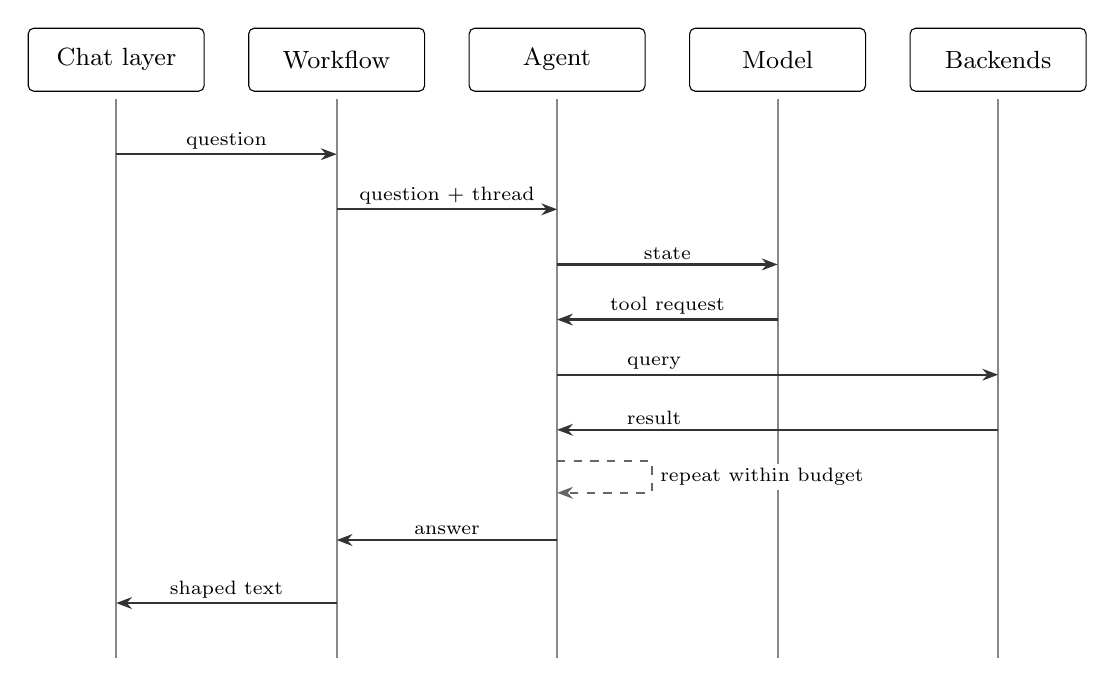
\begin{tikzpicture}[font=\small]

\def\lx{0} \def\wx{28} \def\ex{56} \def\mx{84} \def\tx{112}
\def\ytop{0} \def\ybot{-76}

\foreach \x/\name in {\lx/Chat layer, \wx/Workflow, \ex/Agent, \mx/Model, \tx/Backends} {
  \node[boxn, text width=20mm] at (\x mm, \ytop) {\name};
  \draw[draw=rule, thick] (\x mm, -5mm) -- (\x mm, \ybot mm);
}

\draw[fl] (\lx mm,-12mm) -- node[lbl,above]{\scriptsize question} (\wx mm,-12mm);
\draw[fl] (\wx mm,-19mm) -- node[lbl,above]{\scriptsize question + thread} (\ex mm,-19mm);
\draw[fl] (\ex mm,-26mm) -- node[lbl,above]{\scriptsize state} (\mx mm,-26mm);
\draw[fl] (\mx mm,-33mm) -- node[lbl,above]{\scriptsize tool request} (\ex mm,-33mm);
\draw[fl] (\ex mm,-40mm) -- node[lbl,above,pos=0.22]{\scriptsize query} (\tx mm,-40mm);
\draw[fl] (\tx mm,-47mm) -- node[lbl,above,pos=0.78]{\scriptsize result} (\ex mm,-47mm);

\draw[fldash] (56mm,-51mm) -- (68mm,-51mm) -- (68mm,-55mm) -- (56mm,-55mm);
\node[lbl, right] at (68.5mm,-53mm) {\scriptsize repeat within budget};

\draw[fl] (\ex mm,-61mm) -- node[lbl,above]{\scriptsize answer} (\wx mm,-61mm);
\draw[fl] (\wx mm,-69mm) -- node[lbl,above]{\scriptsize shaped text} (\lx mm,-69mm);

\end{tikzpicture}
\caption{One investigation. The agent mediates between the model and the backends.
The model never reaches a backend directly; it asks the agent to, and reads the
result as text.}
\label{fig:sequence}
\end{figure}

The model issues no network calls: it emits a structured request naming an
operation and its arguments, and the harness looks that name up in the tool set the
agent was built with. An operation outside that set cannot be invoked regardless of
what the model emits, making the tool set an enforcement point, not a convention.

\subsection{Data model}

Two embedded database files sit side by side, each opened by exactly one component.
The operational file holds the watch list (services explicitly monitored regardless
of the general scope rule) and the transition log (one row per observed state
change), written synchronously by the event store. The conversation file holds the
memory component's per-thread checkpoints; nothing else opens it. The split avoids
putting an asynchronous model-turn write and a synchronous polling-task write in
contention for one lock (cost: Section~\ref{sec:decisions}). The transition log is
trimmed on write, retaining ninety days, since a restart loop would otherwise grow
it indefinitely.

% ================================================================ 4
\subsection{The agent}

\subsubsection{The harness}

The agent is one call to the framework's factory, made once and cached, naming the
model client, tool set, operations persona, middleware stack, and conversation
store. Everything the loop does between a question and an answer is the
framework's, shown in Figure~\ref{fig:machine}.

\begin{figure}[H]
\centering
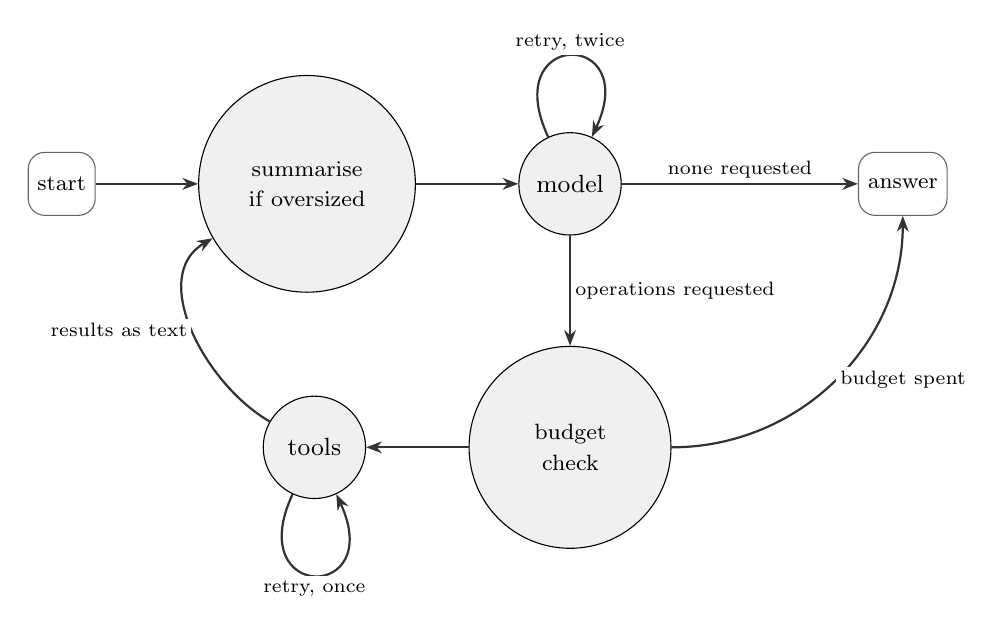
\begin{tikzpicture}[node distance=14mm]

\node[term] (start) {start};
\node[statn, right=13mm of start, text width=24mm] (before) {\footnotesize summarise\\\footnotesize if oversized};
\node[statn, right=13mm of before] (model) {model};
\node[statn, below=14mm of model, text width=22mm] (after) {\footnotesize budget\\\footnotesize check};
\node[statn, left=13mm of after] (tools) {tools};
\node[term, right=30mm of model] (end) {answer};

\draw[fl] (model) to[out=115,in=65,looseness=7] node[lbl,above]{\scriptsize retry, twice} (model);
\draw[fl] (tools) to[out=245,in=295,looseness=7] node[lbl,below]{\scriptsize retry, once} (tools);

\draw[fl] (start) -- (before);
\draw[fl] (before) -- (model);
\draw[fl] (model) -- node[lbl,right]{\scriptsize operations requested} (after);
\draw[fl] (after) -- (tools);
\draw[fl] (tools) to[out=150,in=210] node[lbl,left]{\scriptsize results as text} (before);
\draw[fl] (model) -- node[lbl,above]{\scriptsize none requested} (end);
\draw[fl] (after.east) to[out=0,in=-90] node[lbl,right]{\scriptsize budget spent} (end.south);

\end{tikzpicture}
\caption{The agent as configured. Middleware brackets both nodes: the history is
compressed before the model call and the call retried twice on failure; the tool budget
is enforced after it, and an operation that raises is retried once before its failure
becomes the result text on the return edge. The cycle through the tools and back is the
ordinary loop. Not drawn: each model request carries a thirty-second timeout and the
whole run a sixty-second one, both outside the graph.}
\label{fig:machine}
\end{figure}

Termination is decided by whether the model's most recent message requested any
operations: if so, they run and control returns to the model; if not, that message
is the answer. No separate stopping heuristic, no cap on the answer itself.

\subsubsection{The middleware stack}

Five middleware components, each replacing code this system previously wrote by
hand:

\begin{table}[H]
\centering
\small
\begin{tabular}{|p{32mm}|p{95mm}|}
\hline
\textbf{Middleware} & \textbf{Behaviour} \\
\hline
Model retries & Failed model call retried up to twice before the run is abandoned. \\
\hline
Operation retries & A raising operation retried once before its error is handed on. \\
\hline
Context summarisation & History over the token budget is replaced with a generated
  summary before the model call; may target a cheaper model than the one answering. \\
\hline
Tool budget & A run may spend a fixed number of operations; the call that would
  exceed it, and any sibling call in the same turn, is not executed. \\
\hline
Operation errors & A raising operation becomes an ordinary result carrying the
  failure text, which the model reads and continues from. \\
\hline
\end{tabular}
\end{table}

\subsubsection{The tool budget}

Unbounded loops against a paid or rate-limited endpoint are a liability, so the
number of operations one question may consume is bounded, counting operations
rather than turns (a turn requesting three operations in parallel spends three).
Exceeding the budget produces no error: the run ends with the model's own account
of what it had established, and that partial answer is delivered normally.

\subsubsection{Failure handling}

An operation that raises returns its exception text as the result; a nonexistent
operation the model names is reported as such rather than as a failure ---
the distinction Section~\ref{sec:eval}'s notebooks measure. Retries bound both: a
model call up to three times total, an operation twice. Two time ceilings bound the
run: thirty seconds per model request, sixty seconds overall. The investigation
workflow catches everything above the loop and returns the failure as its answer,
so a caller always gets a string (why: Section~\ref{sec:decisions}).

% ================================================================ 5
\section{Agent state and tools}
\label{sec:memory}

\subsection{Threads}

Conversation state is keyed by the channel or direct message the question arrived in,
so two channels never share history. Omitting a thread id gives a one-shot exchange
with no persistence, incident reports use this path so a report describes the
service, not whatever the channel discussed earlier. There is no interface to read,
write, or delete a stored thread from outside the component that owns it.

\subsection{Durability}

Conversation state lives in its own database file~\cite{sqlite}, so a thread
survives a restart. The storage component holds one connection, opened on first use
inside its event loop and kept for the process lifetime.

\subsection{Bounding a long conversation}

A thread grows without bound while the model's context does not, so history past a
configured token budget is compressed: older turns become a generated summary,
recent turns stay verbatim.

\subsection{Stated limits}

Memory means one conversation replayed per thread: no recall across threads, no
retrieval over past ones. Compression is also lossy by construction, a long
conversation keeps only a summary of its early turns, not the turns themselves.

% ================================================================ 6
\subsection{The tool surface}
\label{sec:tools}

\subsubsection{Composition}

Ten operations are available to the model, covering three backends. Table~\ref{tab:tools}
summarises them.

\begin{table}[H]
\centering\small
\begin{tabularx}{\textwidth}{|l|X|}
\hline
\textbf{Operation} & \textbf{Purpose} \\
\hline
\texttt{list\_services} & Enumerate container names and configured endpoints \\
\hline
\texttt{docker\_status} & State, status and image of one container \\
\hline
\texttt{docker\_logs} & Recent output of one container \\
\hline
\texttt{list\_metric\_names} & Enumerate available metric names \\
\hline
\texttt{get\_label\_values} & Enumerate values of a metric label \\
\hline
\texttt{query\_prometheus} & Instant query for current values \\
\hline
\texttt{query\_prometheus\_range} & Range query for behaviour over a window \\
\hline
\texttt{get\_loki\_label\_values} & Enumerate values of a stream label \\
\hline
\texttt{query\_loki} & Log query over a short recent window \\
\hline
\texttt{query\_loki\_range} & Log query over an explicit window \\
\hline
\end{tabularx}
\caption{The ten read-only operations available to the model.}
\label{tab:tools}
\end{table}

Four of the ten exist purely for discovery, deliberately: a model asked about
resource usage will otherwise query a plausible-sounding metric name that does not
exist, get an empty result, and report usage as zero. Cheap enumeration, with an
instruction to enumerate first, turns that confident wrong answer into a correct one.

\subsubsection{Output discipline}

Every operation returns text and bounds it: results truncate to a fixed length,
enumerations cap at a fixed count, protecting the context window a busy log stream
would otherwise consume outright. Range arguments clamp rather than reject, a
twenty-four-hour log request against a six-hour maximum returns six hours, not an
error.

\subsubsection{Backend notes}

\begin{itemize}
  \item \textbf{Container runtime~\cite{dockerapi}.} Reached over a local socket or
        network address; an unreachable runtime returns an empty list, not an error,
        so a metrics question stays answerable without it. Output framing is parsed
        and stripped before the text reaches the model.
  \item \textbf{Metrics~\cite{promapi,promql}.} Instant queries return current
        values; range queries return a series at a resolution derived from the
        window length, so a thirty-minute and a six-hour query cost about the same
        to transmit and read.
  \item \textbf{Logs~\cite{lokiapi,logql}.} The instant endpoint rejects plain stream
        selectors, so instant queries run as a short-window range query instead.
        Stream labels share no vocabulary with container names or metric labels, so
        the log operations tell the model to enumerate real labels before writing a
        selector.
\end{itemize}

\subsubsection{Input validation}

Label names reach a URL path segment, so they are validated against the backends'
permitted character set before use; a name that fails validation returns an empty
result, not a request. This is a trust boundary, model output is shaped by tool
results that themselves derive from log lines an arbitrary service produced, so it
is not trusted input, and path separators, query markers, and whitespace are all
rejected.

\subsubsection{Read only by construction}
\label{sec:readonly}

The guarantee that the agent cannot act rests on Table~\ref{tab:tools} alone: every
operation is a query, none accepts a state-changing parameter, none reaches a
mutating endpoint. The model is also instructed to recommend actions rather than
perform them, which improves answers but is not the guarantee, instructions
constrain what a model tries, the tool table constrains what it can do.
Section~\ref{sec:socketsec} returns to this for runtime socket access.

% ================================================================ 7
\subsection{Name resolution}
\label{sec:names}

Operators type approximate names, a project prefix here, a role suffix there, hyphens
in one tool and underscores in another. One rule handles it everywhere: a name is
reduced by stripping separators and lowercasing, and a candidate matches if the
reduced query appears inside the reduced candidate.

\begin{enumerate}
  \item \textbf{Exact match wins}, so a service whose name is a prefix of a longer
        one stays addressable.
  \item \textbf{Ambiguity is an error}: several partial matches with no exact match
        fail with a message listing the candidates, rather than silently picking
        one.
\end{enumerate}

The second rule is the one that matters operationally: silently choosing among
matches would produce a believable status report about the wrong service. An
explicit ambiguity message costs one round trip and cannot mislead. The same rule
applies to watch list lookups.

% ================================================================ 8
\section{Monitoring and reporting}

\subsection{The poll cycle}

A single task runs on a configured interval with a floor applied, so a misconfigured
interval cannot produce a tight polling loop. Each cycle reads all container states
and probes each configured HTTP endpoint.

\subsection{Scope}

Container monitoring is off by default. A container is in scope if its name contains
a configured filter substring, or an operator added it to the watch list; an empty
filter puts every container in scope, covering both a single-purpose host and one
sharing unrelated workloads.

\subsection{Transition detection}

The task holds each target's previous observation and compares: running to
not-running is a failure, the reverse a recovery, and endpoints follow the same
pattern over a reachable flag (a non-error response is reachable; an error status, a
connection failure, or a timeout is not). Figure~\ref{fig:transitions} shows the
resulting behaviour, including the case that produces no output.

\begin{figure}[H]
\centering
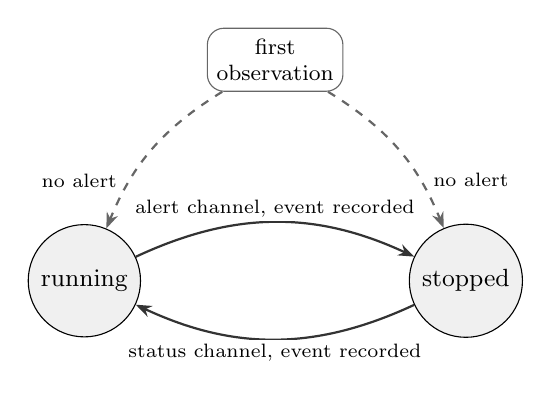
\begin{tikzpicture}[node distance=22mm]

\node[statn] (up) {running};
\node[statn, right=34mm of up] (down) {stopped};
\node[term, above=24mm of $(up)!0.5!(down)$] (new) {first\\observation};

\draw[fl] (up) to[bend left=25] node[lbl,above,pos=0.5]{alert channel, event recorded} (down);
\draw[fl] (down) to[bend left=25] node[lbl,below]{status channel, event recorded} (up);

\draw[fldash] (new) to[bend right=18] node[lbl,pos=0.72,left,xshift=-1mm]{no alert} (up);
\draw[fldash] (new) to[bend left=18] node[lbl,pos=0.72,right,xshift=1mm]{no alert} (down);

\end{tikzpicture}
\caption{Transition handling. Failures and recoveries are routed to different channels.
The first observation of a target establishes a baseline and produces no alert.}
\label{fig:transitions}
\end{figure}

\subsection{Baselining}

The first observation of any target records its state and emits nothing, otherwise
every restart would announce every container already down, training operators to
mute the alert channel. The cost: a container that fails while the agent is not
running is baselined silently once the agent returns, though it still shows, marked
not running, in the report's current-state section.

\subsection{Reading state from the runtime rather than querying metrics}
\label{sec:socket-vs-query}

Liveness could be derived from a metrics query instead, since the metrics server
already tracks whether its scrape targets respond. The runtime is read directly for
two reasons: a metrics-derived signal lags the scrape interval and reports the
transition of a scrape rather than of a process, and if the metrics server itself
restarts, every target it scrapes appears to fail at once, an alert built on metric
queries would announce a total outage when the monitoring system just bounced.
Metrics stay available to the reasoning loop for diagnosis; this decision only
concerns what drives an alert.

\subsection{Endpoint probing}

Endpoint checks catch what runtime inspection cannot: a service on another host,
behind a proxy, or a health path whose success depends on more than the process
being alive.

\subsection{The event log}

Every transition is recorded durably before its alert is dispatched, so a
channel-less environment still accumulates a full history. Live state is held only
in memory and rebuilt each cycle; a target leaving scope drops its state, so a
service returning later is baselined fresh rather than compared to something stale.

% ================================================================ 9
\subsection{Scheduled reporting}

\subsubsection{Schedule}

A single task fires once daily at a configured hour, always publishing the daily
digest and, on one configured weekday, the weekly roll-up too; both are suppressed
with no reports channel configured. There is no catch-up for a missed firing, a
digest delivered late on restart is a distraction rather than a report.

\subsubsection{Periodic status}

A second loop publishes a status snapshot at a configured interval (two hours by
default) to the status channel, reporting current state for every in-scope target;
suppressed with no status channel configured. Unlike a transition alert the snapshot
is a level, it fires whether or not anything changed, so a healthy snapshot is
positive evidence the observer is alive. The first fires on startup and renders the
same current-state section the daily digest opens with.

\subsubsection{Contents}

The daily digest gives current state plus every transition from the preceding
twenty-four hours, in order. The weekly roll-up gives the same current state plus
per-target totals: outage count and cumulative downtime over the window.

\subsubsection{Downtime accounting}

Totals pair each failure event with the recovery that follows it. An unmatched
failure means the target is still down, that outage is measured to the present and
flagged rather than dropped, discarding it would report a three-day outage as no
downtime at all.

\subsubsection{Measured data and generated prose}

Digests separate two kinds of content, and the boundary is enforced. The detail
section is rendered directly from recorded events, the model never sees or rewrites
it, passing an exact value through a language model can only preserve or damage it.
A summary section is generated on top of it for a short narrative before the
numbers, and degrades to the raw detail if the model is unavailable.

\subsubsection{Publication and follow-up}

A report publishes as one unit, one thread where the platform supports it, split
only for the per-message size limit. The report body is written into that thread's
conversation memory, so a reply asking why a service flapped lands in a conversation
that already contains the report.

% ================================================================ 10
\section{Interface and configuration}

\subsection{Commands}

Ten commands are registered through the chat library's application command
tree~\cite{discordpy, discordapi}, listed in Table~\ref{tab:commands}. Commands whose
output concerns only the caller reply privately, so that routine list queries do not
fill a shared channel.

\begin{table}[H]
\centering\small
\begin{tabularx}{\textwidth}{|l|l|X|}
\hline
\textbf{Command} & \textbf{Argument} & \textbf{Effect} \\
\hline
\texttt{status} & none & Current containers and endpoints, summarised \\
\hline
\texttt{investigate} & question & Free-form investigation with all operations \\
\hline
\texttt{report} & service & Structured incident report for one service \\
\hline
\texttt{digest} & period, publish flag & Render a scheduled report immediately \\
\hline
\texttt{containers} & none & Containers grouped by state \\
\hline
\texttt{watching} & none & Endpoints the monitor probes \\
\hline
\texttt{watch} & container & Add a container to the watch list \\
\hline
\texttt{unwatch} & container & Remove a container from the watch list \\
\hline
\texttt{watchlist} & none & Containers currently watched \\
\hline
\texttt{help} & none & List the commands \\
\hline
\end{tabularx}
\caption{The command set.}
\label{tab:commands}
\end{table}

\subsection{Conversational access}

A direct message, or a mention in a channel the agent can see, routes through the
same investigation path as the explicit command, mention markup stripped first; a
mention with no question prompts for one. Because the thread id is the channel, an
operator can hold an ordinary exchange, ask, then why, then for evidence, without
restating the subject.

\subsection{Output shaping}
\label{sec:shaping}

Model output needs two corrections before it is fit to send: the platform's
restricted markdown dialect shows heading syntax literally and renders tables as
pipe-character rows, so headings are rewritten to bold text and tables to labelled
bullet lines (code fences are exempt); and answers over the platform's message-length
cap are split, preferring line boundaries so a split does not land inside a word.

\subsection{Log forwarding}

Informational-and-above application logs forward to a configured channel, making the
agent observable through the interface it serves. Library records are dropped, to
avoid the feedback loop of a sent message logging an event that sends a message;
forwarding is asynchronous and batched for one second per message; the queue is
bounded at a thousand records, beyond that records drop rather than growing memory.
What reaches the channel is the operational trail, transitions, alerts, reports, and
per-question call counts and duration, not debug noise. A drain failure is written to
standard error rather than logged, to avoid feeding the forwarder that failed.

\subsection{Failure must be visible}
\label{sec:silent}

The chat library logs a handler exception to its own logger, exactly the logger
excluded from forwarding above, so a failure answering a mention would go unseen and
the agent would simply not reply. Message handling is instead wrapped in a workflow
that always sends an explicit reply on failure. Section~\ref{sec:decisions} states why
an error message beats silence.

% ================================================================ 11
% ================================================================ 12
\section{Deployment}

\subsection{Packaging}

One container image, on a slim Python~\cite{python} base, with dependencies resolved
from a lock file~\cite{uv} and installed in a layer built before the application
source is copied, so a source change reuses the cached dependency layer. The compose
description~\cite{compose} runs two services from that image: the Discord bot, and a
read-only HTTP API mirroring the same status, investigation, report, and watch-list
workflows, every route but \texttt{/health} guarded by an optional key header. The
API binds loopback only by default; host networking would otherwise expose it on the
LAN.

\subsection{The observability backends}

Neither service starts the metrics server or log store; both are pre-existing
infrastructure addressed by configuration, and each is independently optional ---
with either address unset, its operations drop from the tool set. The log store's
labels are set by whatever ships logs into it, not by this system, which is why label
values are discovered rather than hard-coded (Section~\ref{sec:tools}).

\subsection{Networking and persistence}

The agent shares the host's network namespace, reaching the backends and the model
endpoint at local addresses; bridge-networked components reach it through the host
gateway instead of by service name. The storage file lives on a mounted directory so
the watch list, transition history, and conversation threads survive container
replacement --- losing that directory loses the reporting history irrecoverably.

\subsection{Runtime socket access}
\label{sec:socketsec}

The agent needs the container runtime's API socket to read container state and
output. The socket is mounted read-only, but that flag governs only the socket file:
the API reachable through it stays fully writable, and access to it is equivalent to
root on the host.

\subsection{Operating the system}

The process restarts automatically unless explicitly stopped, and shutdown closes the
conversation store before the event loop ends. The log channel and the container's
own output both carry informational records and above in real time; the container
output is where to look when the chat connection itself is the problem.
Transport-level logging stays pinned to warnings to avoid flooding both destinations.

% ================================================================ 13
\section{Evaluation}

\subsection{Model behaviour evaluation}
\label{sec:eval}

Tests verify the code, not whether a given model chooses sensible operations, and a
model substitution changes that while leaving every test passing. A separate notebook
harness~\cite{jupyter} addresses this, read by a human rather than asserted on. Seven
notebooks each isolate one operation, binding it plus the discovery calls it requires
and nothing else, driving the production agent through a shared instrumented entry
point so every run's transcript records the same fields: system prompt, bound
operations, each call and result, token cost, and duration.

Each isolation notebook asks two questions: one answerable with the bound operations,
and one requiring evidence from a backend that isn't bound --- the more informative
case, since it measures whether the model states the limit or fabricates an answer
(a service reported healthy from name enumeration alone, for instance). Runs are
thread-isolated by default, so re-running a case can't replay a prior conversation
into the model's context; continuing a thread is an explicit opt-in reserved for
cases where memory is itself the subject.

An eighth notebook drives the production agent directly with memory, exercising what
isolation cannot: which backend the model selects when nothing is withheld, and
whether context carries across a follow-up on the same thread versus a fresh one. A
suite runner executes every notebook's cases in one process against whichever model
is configured, and an analysis script reads the transcripts into a per-case
comparison, per-model averages, and token cost by operation.

\subsubsection{A conclusive model comparison}
\label{sec:eval-comparison}

After the tool-name hallucination incident described in Section~\ref{sec:silent} was
traced to a stale in-process prompt and a workflow that mandated operations which were
not bound, both defects were fixed, and the full suite --- seventeen cases: two per
isolation notebook plus the three memory cases --- was run against the two candidate
models with live backends. Tables~\ref{tab:per-case-inscope}--\ref{tab:per-case-memory} give the full per-case record;
Table~\ref{tab:model-comparison} summarises it; Table~\ref{tab:tool-cost} attributes
token cost to each operation.

\begin{table}[H]
\centering
\footnotesize
\begin{tabular}{|p{3.4cm}|p{5.6cm}|p{5.6cm}|}
\hline
\textbf{In-scope case} & \textbf{gemma-4-31b-it} & \textbf{marconi-llm} \\
\hline
list services & 1v · 1{,}326t · 9.5s & 1v · 1{,}960t · 4.0s \\
\hline
status & 1v · 1{,}349t · 8.8s & 1v · 1{,}814t · 2.9s $\emptyset$ \\
\hline
logs & 1v · 3{,}108t · 9.0s & 1v · 3{,}800t · 4.0s \\
\hline
instant query & 1v · 2{,}125t · 12.1s & 1v · 2{,}494t · 2.6s \\
\hline
range query & 1v · 4{,}820t · 8.9s & 2v · 7{,}741t · 4.0s \\
\hline
loki errors & 3v · 9{,}904t · 27.5s & 10v · 49{,}921t · 19.7s $\emptyset$ \\
\hline
loki range & 2v · 4{,}730t · 22.0s & 13v L · 17{,}139t · 34.5s \\
\hline
\end{tabular}
\caption{Per-case results, in-scope cases. v = valid tool calls, i = invalid (hallucinated) calls, t = total tokens; $\emptyset$ = empty final answer, L = call-limit exit.}
\label{tab:per-case-inscope}
\end{table}

\begin{table}[H]
\centering
\footnotesize
\begin{tabular}{|p{3.4cm}|p{5.6cm}|p{5.6cm}|}
\hline
\textbf{Out-of-scope case} & \textbf{gemma-4-31b-it} & \textbf{marconi-llm} \\
\hline
health, discovery only & 1v/1i · 5{,}224t · 267s & 1v · 1{,}783t · 2.7s \\
\hline
logs, status only & 0v · 677t · 7.3s & 1v · 2{,}780t · 9.9s \\
\hline
health, logs only & 1v/1i · 5{,}113t · 19.8s & 1v · 3{,}836t · 4.3s \\
\hline
trend, instant only & 7v · 10{,}507t · 34.3s & 1v · 2{,}681t · 4.8s \\
\hline
logs, prom only & 0v · 748t · 6.2s & 0v · 1{,}563t · 5.3s \\
\hline
CPU, loki only & 0v · 977t · 12.6s & 0v · 1{,}513t · 5.1s \\
\hline
health, loki only & 3v · 9{,}223t · 20.4s & 2v · 5{,}220t · 4.7s \\
\hline
\end{tabular}
\caption{Per-case results, out-of-scope cases. Same legend as Table~\ref{tab:per-case-inscope}.}
\label{tab:per-case-outscope}
\end{table}

\begin{table}[H]
\centering
\footnotesize
\begin{tabular}{|p{3.4cm}|p{5.6cm}|p{5.6cm}|}
\hline
\textbf{Memory case} & \textbf{gemma-4-31b-it} & \textbf{marconi-llm} \\
\hline
broad "anything wrong?" & 12v L · 3{,}269t · 15.4s & 11v L · 3{,}695t · 3.4s \\
\hline
follow-up, same thread & 0v · 3{,}010t · 25.6s & 1v · 5{,}104t · 3.8s \\
\hline
follow-up, fresh thread & 0v · 1{,}585t · 11.3s & 11v L · 4{,}102t · 6.3s \\
\hline
\end{tabular}
\caption{Per-case results, broad and follow-up (memory) cases. Same legend as Table~\ref{tab:per-case-inscope}.}
\label{tab:per-case-memory}
\end{table}

\begin{table}[H]
\centering
\small
\begin{tabular}{|l|r|r|}
\hline
 & \textbf{gemma-4-31b-it} & \textbf{marconi-llm} \\
\hline
Valid calls per run            & 2.00 & 3.41 \\
\hline
Hallucinated calls per run     & 0.12 (2 of 17 runs) & \textbf{0.00} \\
\hline
Tokens per run                 & 3{,}982 & 6{,}891 \\
\hline
Duration per run               & 30.5 s & \textbf{7.2 s} \\
\hline
Runs ending at the call limit  & 1 & 3 \\
\hline
Empty final answers            & \textbf{0} & 2 \\
\hline
\end{tabular}
\caption{Full-suite comparison, seventeen cases per model, live backends, 2026-08-27.}
\label{tab:model-comparison}
\end{table}

\begin{table}[H]
\centering
\small
\begin{tabular}{|l|r|r|}
\hline
\textbf{Operation} & \textbf{gemma avg · total} & \textbf{marconi avg · total} \\
\hline
\texttt{query\_loki} & 5{,}814 · 11.6k & \textbf{10{,}484 · 73.4k} \\
\hline
\texttt{query\_loki\_range} & 4{,}821 · 14.5k & 3{,}289 · 26.3k \\
\hline
\texttt{get\_loki\_label\_values} & 1{,}859 · 5.6k & 2{,}119 · 21.2k (10 calls) \\
\hline
\texttt{query\_prometheus} & 2{,}197 · 17.6k & 3{,}599 · 7.2k \\
\hline
\texttt{docker\_logs} & 3{,}676 · 7.4k & 3{,}634 · 7.3k \\
\hline
\texttt{query\_prometheus\_range} & 4{,}710 · 4.7k & 6{,}523 · 6.5k \\
\hline
\texttt{list\_services} & 1{,}506 · 6.0k & 2{,}572 · 10.3k \\
\hline
\texttt{list\_metric\_names} & 1{,}932 · 1.9k & 2{,}380 · 4.8k \\
\hline
\texttt{docker\_status} & 282 · 3.1k & 384 · 8.4k \\
\hline
\end{tabular}
\caption{Average tokens per invocation and total tokens spent across the suite, by operation.}
\label{tab:tool-cost}
\end{table}

The tables carry the numbers; four qualitative reads don't reduce to them:

\begin{itemize}
  \item \textbf{Boundary respect.} Bound to instant queries only, gemma faked a
        thirty-minute trend with seven improvised calls (case 04); marconi-llm named
        the limit and stopped. Both refused a logs request cleanly when bound to
        metrics.
  \item \textbf{Hallucination residue.} gemma invented one operation name per run
        before self-correcting, a different name each time --- a model prior, not a
        prompt defect. marconi-llm invented none.
  \item \textbf{Budget exhaustion.} Both models exhausted the ten-call budget polling
        \texttt{docker\_status} once per container (case 08) and were cut off with no
        summary. Fix: aggregate queries, or a larger budget for broad questions.
  \item \textbf{Empty-answer defect.} marconi-llm returned
        \texttt{finish\_reason=stop} with no text twice in seventeen runs. Suspected
        proxy or streaming quirk; undiagnosed.
\end{itemize}

\noindent\textbf{Conclusion.} Adopt marconi-llm for the agent loop, conditional on
diagnosing and defending against the empty-answer defect (a retry-on-empty rule makes
the failure survivable even before the cause is found); retain gemma as fallback. The
token advantage of gemma's shorter runs is outweighed by marconi-llm's 4.3$\times$
speed, its perfect boundary behaviour, and its zero operation hallucinations. The
comparison is a single snapshot per case, and the empty-answer defect is intermittent
by nature; the suite should be repeated three times per model before the substitution
is final.

% ================================================================ 14
\section{Design decisions and outcome}
\label{sec:decisions}

% ================================================================ 15
\subsection{Limitations and extensions}

\subsubsection{Limitations}

\begin{enumerate}
  \item \textbf{Answer quality tracks model quality.} The system supplies evidence
        and structure; the reasoning is the model's. The evaluation harness exists
        because this cannot be tested automatically.
  \item \textbf{Memory does not span conversations.} A thread is a conversation;
        nothing is recalled across threads.
  \item \textbf{Long conversations keep a summary, not a record.} Past the context
        budget, early turns are replaced by generated prose --- a detail mentioned
        once survives only if the summarising model kept it.
  \item \textbf{Monitoring has a blind interval.} The first observation after a
        restart is a baseline, so a failure during downtime is never announced,
        though it remains visible in the next report.
  \item \textbf{Missed report firings are skipped.} No catch-up: an agent down at
        the scheduled hour omits that day's digest.
  \item \textbf{The deployment is single tenant.} Authorisation is whatever the chat
        workspace enforces; anyone who can message the agent can query every service
        it can see.
  \item \textbf{Alerting observes state, not thresholds.} A service running but
        degraded produces no alert unless an HTTP probe happens to catch it.
\end{enumerate}

\subsubsection{Possible extensions}

\begin{enumerate}
  \item \textbf{Threshold alerting} would fill the degraded-but-running gap, with
        care to avoid the correlated-failure problem (Section~\ref{sec:socket-vs-query}).
  \item \textbf{Persisting monitor state} would close the blind interval by comparing
        the first post-restart observation against the last one before it.
  \item \textbf{Write operations}, if ever added, belong in a distinct tool set
        behind an explicit approval step, not folded into the existing surface --- the
        value of Section~\ref{sec:readonly}'s guarantee is in it being absolute.
  \item \textbf{Additional backends} fit the existing pattern: a client, a set of
        query operations, an entry in the tool list. Nothing else changes.
\end{enumerate}

% ================================================================ 16
\subsection{Conclusion}

The system automates a repetitive part of operations work: gathering evidence from
three separate systems and correlating it into an account of what happened, through a
language model given a fixed set of query operations and reached from the chat
workspace an operator already uses.

Its most consequential property is what it cannot do. No operation available to the
model changes anything, placing the guarantee in the composition of the tool set
rather than in instructions the model may disregard --- the constraint that lets an
autonomous reasoning loop run against a live environment while the worst outcome
stays an incorrect answer.

The remaining design follows from taking failure seriously in a system whose central
component is probabilistic:

\begin{itemize}
  \item \textbf{The reasoning loop is bounded}, and returns a partial summary instead
        of an error when the bound is reached.
  \item \textbf{Operation failures become evidence} rather than exceptions.
  \item \textbf{Report figures are rendered from recorded data} and never passed
        through the model, which restricts generation to the parts where fluency helps.
  \item \textbf{Monitoring baselines before it alerts}, because an alert stream that
        cries wolf on every restart is worse than none.
\end{itemize}

Every one of these choices costs something, and Section~\ref{sec:decisions} states the
costs alongside the reasoning.


% ================================================================ REFERENCES
\clearpage
\addcontentsline{toc}{section}{References}
% thebibliography emits its own \section*; restore the plain definition so the
% per-section \clearpage does not split the heading from the entries.
\begingroup
\let\section\stdsection
\begin{thebibliography}{99}
\setlength{\itemsep}{4pt}

\bibitem{python}
Python Software Foundation, ``Python 3.13 documentation.'' [Online].
Available: \url{https://docs.python.org/3.13/}. [Accessed: Aug. 18, 2026].

\bibitem{langchain}
LangChain, Inc., ``LangChain Python documentation: agents.'' [Online].
Available: \url{https://docs.langchain.com/oss/python/langchain/agents}. [Accessed: Aug. 25, 2026].

\bibitem{openai}
OpenAI, ``Chat Completions API reference.'' [Online].
Available: \url{https://platform.openai.com/docs/api-reference/chat}. [Accessed: Aug. 18, 2026].

\bibitem{discordpy}
Rapptz and contributors, ``discord.py documentation.'' [Online].
Available: \url{https://discordpy.readthedocs.io/}. [Accessed: Aug. 18, 2026].

\bibitem{discordapi}
Discord, Inc., ``Discord Developer Portal: API reference.'' [Online].
Available: \url{https://discord.com/developers/docs/}. [Accessed: Aug. 18, 2026].

\bibitem{httpx}
Encode OSS Ltd., ``HTTPX: a next-generation HTTP client for Python.'' [Online].
Available: \url{https://www.python-httpx.org/}. [Accessed: Aug. 18, 2026].

\bibitem{sqlite}
SQLite Consortium, ``SQLite documentation.'' [Online].
Available: \url{https://www.sqlite.org/docs.html}. [Accessed: Aug. 18, 2026].

\bibitem{dockerapi}
Docker, Inc., ``Docker Engine API reference.'' [Online].
Available: \url{https://docs.docker.com/reference/api/engine/}. [Accessed: Aug. 18, 2026].

\bibitem{compose}
Docker, Inc., ``Docker Compose documentation.'' [Online].
Available: \url{https://docs.docker.com/compose/}. [Accessed: Aug. 18, 2026].

\bibitem{promapi}
Prometheus Authors, ``Prometheus HTTP API.'' [Online].
Available: \url{https://prometheus.io/docs/prometheus/latest/querying/api/}. [Accessed: Aug. 18, 2026].

\bibitem{promql}
Prometheus Authors, ``Querying Prometheus: PromQL basics.'' [Online].
Available: \url{https://prometheus.io/docs/prometheus/latest/querying/basics/}. [Accessed: Aug. 18, 2026].

\bibitem{lokiapi}
Grafana Labs, ``Grafana Loki HTTP API.'' [Online].
Available: \url{https://grafana.com/docs/loki/latest/reference/loki-http-api/}. [Accessed: Aug. 18, 2026].

\bibitem{logql}
Grafana Labs, ``LogQL: Loki query language.'' [Online].
Available: \url{https://grafana.com/docs/loki/latest/query/}. [Accessed: Aug. 18, 2026].

\bibitem{uv}
Astral Software, Inc., ``uv: Python packaging documentation.'' [Online].
Available: \url{https://docs.astral.sh/uv/}. [Accessed: Aug. 18, 2026].

\bibitem{jupyter}
Project Jupyter, ``Jupyter documentation.'' [Online].
Available: \url{https://docs.jupyter.org/}. [Accessed: Aug. 18, 2026].

\end{thebibliography}
\endgroup


\end{document}
